\subsection{Onshore wind (1,584~\$/kW)}\label{sec:onwind}
Onshore wind can provide low-cost clean electricity and complement solar's intermittency or low regional suitability.

The CAPEX of 1,584~\$/kW is the 2025 value of the DEA catalogue \citep{dea} as carried by technology-data \citep{technologydata}.
It lies well above the global average of 1,041~\$/kW that IRENA reports for 2024 (Figure~\ref{fig:onwind}).

The global average is dominated by China, which installs most new wind at much lower turbine and construction costs (856~\$/kW in 2024), while the DEA describes Danish projects.
The rest of the world is closer to Europe than to China \citep[Table~2.1]{irena2025}: India builds at 1,110~\$/kW, but most other regions at 1,240--1,490~\$/kW (Africa, Oceania, Brazil, the rest of the Americas), the US at 1,568 and Europe at 1,659~\$/kW, and the rest of Asia, including Japan and Korea, at 1,912~\$/kW.
Our value thus fits most regions outside China and India.
DEA turbines also have large rotors for their rating, which costs more per kW but yields a higher capacity factor.
Lower regional CAPEX may be needed for China and India.

\begin{figure}[htbp]\centering
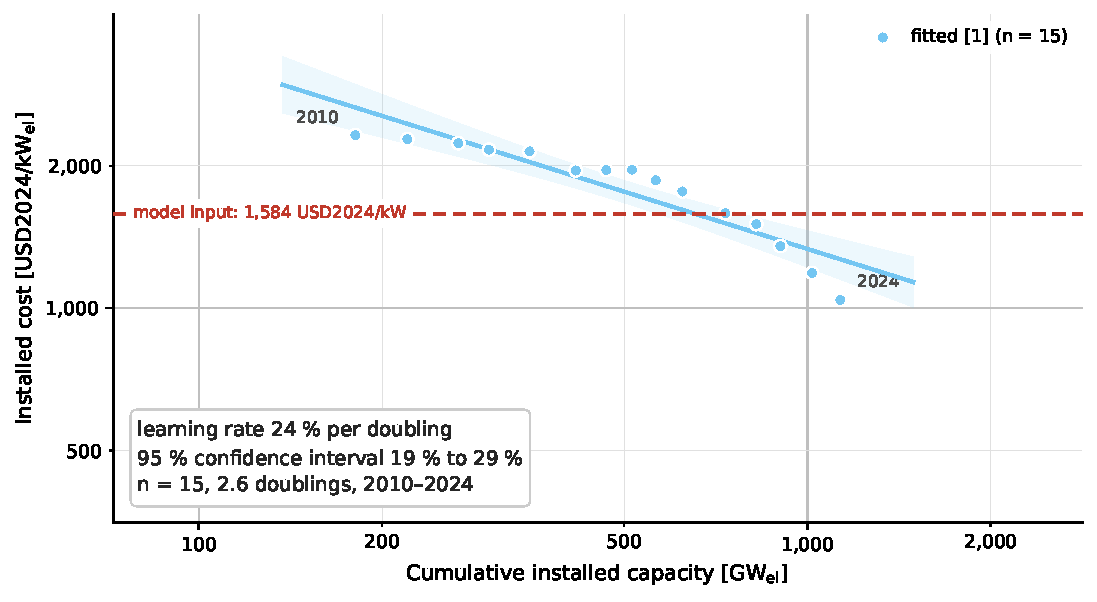
\includegraphics[width=\textwidth]{../../../misc-quarter1/technology-costs/figures/learning/onwind.pdf}
\caption{Installed cost of onshore wind against cumulative capacity.
Source: [1] \citet{irena2025}, fitted.
Dashed red line: the model input.}\label{fig:onwind}
\end{figure}

We apply an exogenous cost path from the DEA projections \citep{dea}.

O\&M and the 28.5-year lifetime come from technology-data \citep{technologydata}.
Existing capacity is Ember's 2024 wind total minus the offshore fleet reported by the Global Wind Energy Council \citep{gwec2025}.

Wind resources vary even more than solar radiation (Figure~\ref{fig:onwind-maps}).
The best sites, in Patagonia, the British Isles, the US and southern Australia, reach capacity factors of 0.4--0.6 and a levelised cost of 30--45~\$/MWh.

\begin{figure}[htbp]\centering
\begin{subfigure}[t]{0.49\textwidth}\centering
\includegraphics[width=\linewidth]{../build/figures/onwind_cf.pdf}
\caption{Annual mean capacity factor}
\end{subfigure}\hfill
\begin{subfigure}[t]{0.49\textwidth}\centering
\includegraphics[width=\linewidth]{../build/figures/onwind_lcoe.pdf}
\caption{Levelised cost of electricity}
\end{subfigure}
\caption{Onshore wind, 0.5$^\circ$ cells.
Left: annual mean capacity factor from ERA5 weather of 2011 \citep{hersbach2020}, as converted by \href{https://model.energy}{model.energy} \citep{modelenergy}.
Right: the resulting levelised cost with the costs of Table~\ref{tab:costs} at a 7\,\% real discount rate.}\label{fig:onwind-maps}
\end{figure}

Regional differences in the cost of capital could be considered: in low- and middle-income countries, high financing costs add on average 24~\$/MWh to the levelised cost of onshore wind \citep{hatton2026}.
